To reduce animation artifacts and afford performative behaviors, the stylized and performative gaze methods deliberately direct the characters's gaze shifts toward locations that are different from the intended gaze targets. In addition, stylized gaze methods produce eye poses and kinematics that are impossible in biologically accurate human gaze. Previous studies on gaze perception have shown that people are generally imprecise at judging gaze direction~\citep{argyle1976gaze}, suggesting that these deviations from normal human gaze might not worsen judgments that already show very high variability. Therefore, we conducted evaluation to determine whether these deviations affected the communicative accuracy and perceived naturalness of gaze shifts adapted using our methods compared with the original gaze shift model~\ref{cha:GazeShiftModel}.

\subsection{Study Design}

The study followed a three-by-one, between-participants design. The experimental conditions included gaze shifts performed by (1) \textit{original}: a character with human proportions following the original gaze shift model, (2) \textit{original stylized}: a character with a stylized design following the original gaze shift model, and (3) \textit{adapted}: the stylized character with our adaptation methods applied. We chose a between-participants design to minimize transfer effects. Figure~\ref{fig:StudyTask} illustrates the two characters used in the study. The \textit{adapted} condition involved performative gaze shifts with an eye-alignment parameter of $0.85$.

\begin{figure}
\centering
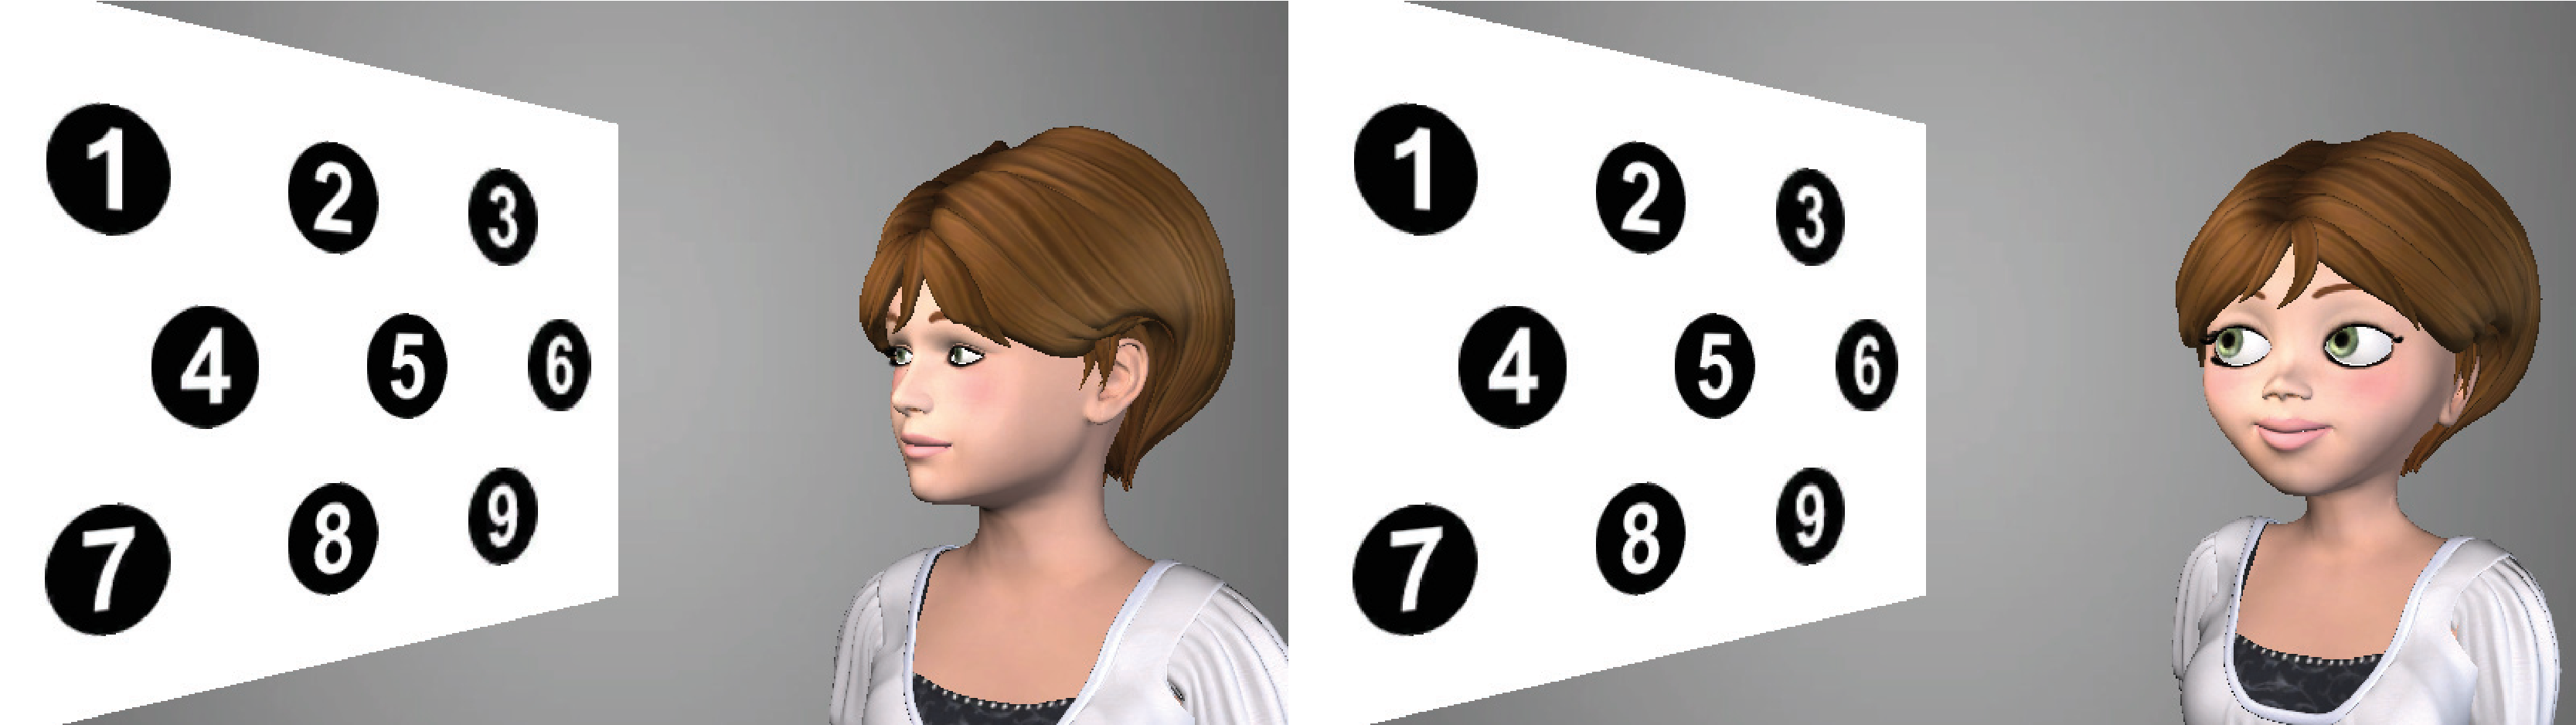
\includegraphics[width=0.9\textwidth]{stylizedgaze/Figures/StudyTask-small.pdf}
\caption{Stills from videos in our study. Left: Realistically-proportioned character. Right: Stylized character.}
\vspace{-12pt}
\label{fig:StudyTask}
\end{figure}

\subsection{Task}

Participants in the study watched a series of videos of the character shifting its gaze toward numbered targets arranged on a whiteboard and tried to identify the target toward which the character was looking (Figure~\ref{fig:StudyTask}). The character was positioned in front of the camera, approximately $1 m$/$3.3 ft$ away and slightly to the right. The whiteboard was positioned on the character's right and oriented so that the viewer and the character could comfortably see the targets.

\subsection{Procedure}

We recruited 48 participants using the Amazon Mechanical Turk crowd-sourcing service. Each participant was paid U.S. \$1 for their participation.

After recruitment, each participant reviewed and agreed to a consent form. Following informed consent, the participants viewed a sequence of $22$ videos. In each video, the character shifted its gaze toward a randomly selected target from among nine targets on the whiteboard. After watching each video, the participants were asked to determine the target toward which the character was looking and provide their answer in a text field. Each video was approximately ten seconds in length. At the beginning of each video, the character looked toward the camera and nodded. It then shifted its gaze toward one of the targets, maintained its gaze at the target for two seconds, and then looked back toward the viewer.

At the end of the study, each participant filled out a questionnaire to provide subjective evaluations of the character. The study took approximately ten minutes.

To ensure the quality of the experimental data, we followed crowd-sourcing best practices \citep{kittur2008crowdsourcing}. For example, all participants were shown two training and acclimation videos, where the correct gaze target would light up during the gaze shift. Data from participants who failed to correctly identify the target were discarded. We also restricted the task to workers with high approval rates and tracked statistics such as task completion time and screen resolution.

\subsection{Measures}

The dependent variables in our study were \textit{communicative accuracy}, \textit{naturalness of eye movements}, \textit{lifelikeness}, and \textit{appeal}. Communicative accuracy was measured as the percentage of correctly identified gaze targets. Naturalness of eye movements, lifelikeness, and appeal were measured using a questionnaire. Participants rated each item in the questionnaire using seven-point rating scales ($1 = not likable$; $7 = likable$). The lifelikeness scale included three items that measured lifelikeness, humanlikeness, and believability ($Cronbach's \alpha = 0.799$), while the appeal scale included four items that measured charisma, attractiveness, cuteness, and likability ($Cronbach's \alpha = .796$).

Data analysis included one-way analysis of variance (ANOVA) tests, following the guidelines suggested by~\citet{julnes1989analysis} for establishing a ``no difference'' in comparisons, particularly an alpha level of $0.25$ (i.e., $p > .25$) to control for Type II errors.
%http://deepblue.lib.umich.edu/bitstream/2027.42/67182/2/10.1177_0193841X8901300604.pdf

\subsection{Results}

\begin{figure}
\centering
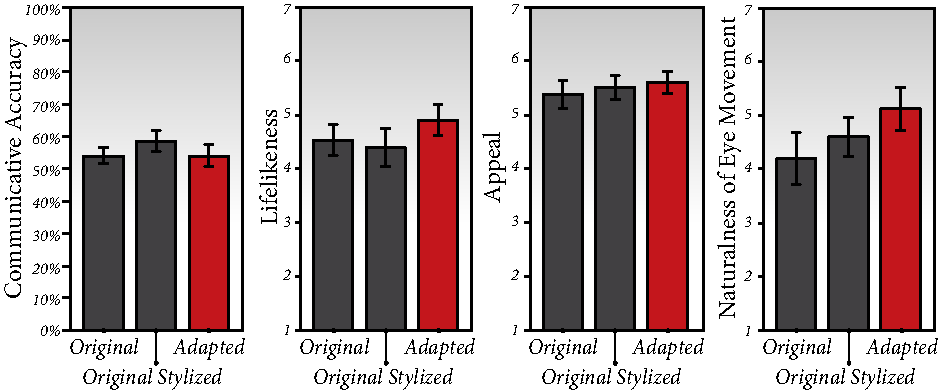
\includegraphics[width=1\textwidth]{stylizedgaze/Figures/Results.pdf}
\caption{Results for communicative accuracy, lifelikeness, appeal, and naturalness of eye movements. Data on gaze shifts adapted using the stylized and performative gaze methods are shown in red.}
\label{fig:StudyResults}
\end{figure}

Results for all the measures are illustrated in Figure \ref{fig:StudyResults}. The mean accuracies in the original, original stylized, and adapted conditions were $54.0\%$, $58.6\%$, and $54.0\%$, respectively. The statistical analysis of the data found no significant effect of our manipulation on accuracy, $F(2,45) = 0.83$, $p = 0.44$. These rates are considerably better than chance, which we expect to be closer to 1/3 than 1/9, as our informal analysis suggests that it is easy to determine toward which row is being looked, and are consistent with results from previous work~\citep{argyle1976gaze,goldberg1969visual,andrist2012designing}. Pairwise contrast tests also found no differences between the original and original stylized conditions, $F(1,45) = 0.00$, $p = 1.00$, or between the original and adapted conditions, $F(1,45) = 1.20$, $p = 0.28$. These results suggest that the adaptation methods retain the communicative accuracy of the original gaze shift model.

Our analysis revealed no significant effect of our manipulation on the perceived naturalness of eye movements, $F(2,45) = 1.27$, $p = 0.29$. Contrast tests also found no differences between the original and original stylized conditions, $F(1,45) = 0.53$, $p = 0.47$, or between the original and adapted conditions, $F(1,45) = 2.52$, $p = 0.12$, suggesting that the adaptation methods preserve the naturalness of eye movements generated by the original model.

We found no significant effects of our manipulation on the lifelikeness measure, $F(2,45) = 0.69$, $p = 0.51$. Pairwise contrasts showed no differences between the original and original stylized conditions, $F(1,45) = 0.10$, $p = 0.75$, or original stylized and adapted conditions, $F(1,45) = 0.64$, $p = 0.43$. Similarly, we found no effects of our manipulation on the appeal measure, $F(2,45) = 0.25$, $p = 0.78$. No differences appeared in pairwise contrast tests between the original and original stylized conditions, $F(1,45) = 0.18$, $p = 0.68$, or original stylized and adapted conditions, $F(1,45) = 0.49$, $p = 0.49$.

Overall, the results suggest that stylized and performative gaze methods do not change the communicative accuracy of the character's gaze shifts or the subjective evaluations of the character. While we speculate that the removal of animation artifacts may improve the character's appeal, such effects are unlikely to appear in short, focused tasks. Future studies might further explore how stylized and performative gaze adaptations might shape subjective impressions of the character in longer, more realistic scenarios. 